\newpage
\section{Pembuatan Sistem Face Recognition}
Prose pertama untuk melakukan pengenalan wajah yaitu dengan mengumpulkan dataset yang akan di \emph{training} dengan menangkap citra wajah pada saat awal deteksi wajah yang akan 
disimpan dan dikumpulkan berdasarkan id yang telah dimasukkan user. Setelah dataset terkumpul, selanjutnya sistem akan melakukan \emph{training data} untuk mengenali wajah berdasarkan id. 
Kemudian proses penenalan wajah pun dilakukan dengan mendeteksi wajah mengunakan algoritma Haar-cascade classifier, lalu sistem akan melakukan pencocokan dengan menggunakan fitur LBPH 
untuk mencocokan wajah yang terdeteksi dengan dataset yang sudah di\emph{training} sebelumnya.
\begin{enumerate}[1.]
\item Proses mengumpulkan dataset dengan

- Memasukan library openCV, yaitu \textbf{cv2}
\begin{figure}[h!]
    \centering
    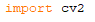
\includegraphics[width=0.3\linewidth]{images/fr_1.PNG}
    \caption{Memasukan library openCV}
\end{figure}

-  Proses face detection, untuk melakukan proses deteksi wajah akan menggunakan algoritma \emph{haarcascade}. Dengan fungsi \textbf{cv2.CascadeClassifier} pada baris pertama, 
pada baris kedua merupakan fungsi openCV untuk memasukan video atau kamera yang terhubung dengan \textbf{cv2.VideoCapture()}
\begin{figure}[h!]
    \centering
    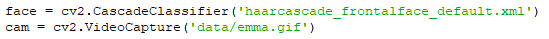
\includegraphics[width=0.85\linewidth]{images/fr_2.PNG}
    \caption{Proses face detection}
\end{figure}

- Menambahkan variabel 'jumlah' yang dimulai dari 0 untuk menyimpan data perulangan pengambilan gambar dataset
dan juga pada baris selanjutnya ada variabel 'id' wadah masukan user untuk id dataset
\begin{figure}[h!]
    \centering
    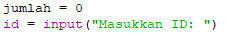
\includegraphics[width=0.5\linewidth]{images/fr_3.PNG}
    \caption{Tambah variabel}
\end{figure}
\newpage
- Membaca video atau kamera yang sudah dimasukkan sebelumnya dengan fungsi \textbf{read()}, dan untuk mengubah warna citra menjasi hitam-putih/grayscale
dengan fungsi \textbf{cv2.cvtColor}
\begin{figure}[h!]
    \centering
    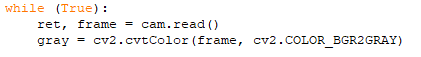
\includegraphics[width=0.85\linewidth]{images/fr_4.PNG}
    \caption{Membaca video dan merubah warna citra}
\end{figure}

\item Proses training dataset
\item Testing aplikasi: Proses pengenalan wajah dengan metode \emph{Local Binary Patter Histogram(LBPH)}
\end{enumerate}
